\documentclass{article}
\usepackage{ctex}
\usepackage{amsmath}
\usepackage{graphicx}
\usepackage{wrapfig}
\usepackage{caption}
\usepackage[top=0.8in, bottom=0.8in,left=0.8in, right=0.8in]{geometry}
\usepackage{float} 
\usepackage{subfigure}
\usepackage{subcaption}
\usepackage{bm}
\xeCJKsetup{CJKmath=true} 

\begin{document}
\section*{Arago圆盘(40分)}
\begin{wrapfigure}{r}{7cm}
	\vspace{-15pt}    % 对应高度1
	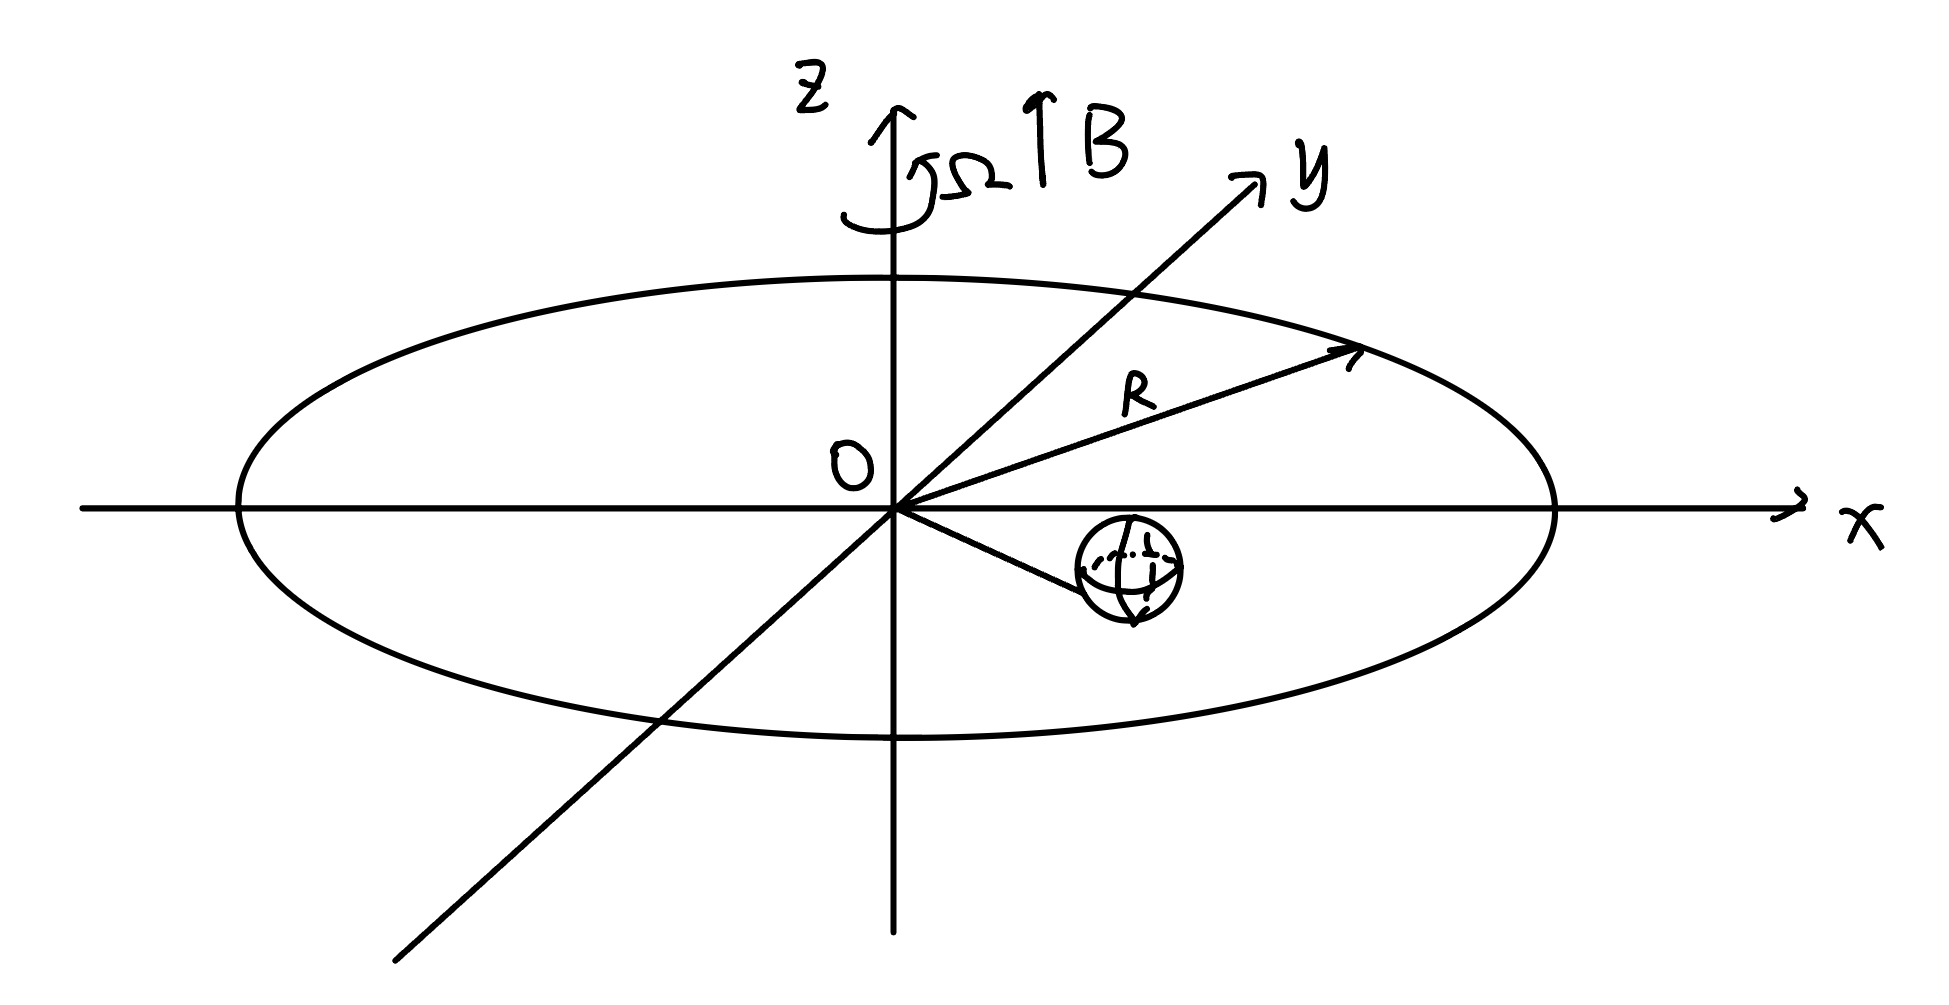
\includegraphics[width=7cm]{img/1.jpeg}\\
	\vspace{-15pt}    % 对应高度2
	\caption{}
	\vspace{-15pt}    % 对应高度3
\end{wrapfigure}
高二这次期中考考了一个有关于Arago圆盘的选择题,小H同学对J老师的解释不是很满意,于是他尝试自己着手计算一下。\par
将小磁针认为是一个磁偶极子,大小为$\mu$。下方$h$处有一个带电薄圆盘质量为$m$,半径为$R$,以$\omega$转动,现固定小磁针。
\begin{itemize}
    \item[(1)]求圆盘上的磁感应分布。 
    \item[(2)]将下方带电薄圆盘以$\Omega$恒定速度转动,求小磁针受到的力矩。
    % \item[(2)]现释放小磁针,并解除下方维持带电薄圆盘匀速转动的力矩,求两者共速后的共同角速度$\Omega$.
\end{itemize}
\par
补充:磁偶极子的场
\[
\vec{B}=\dfrac{\mu}{4\pi}\dfrac{(3(\vec{\mu}\cdot\hat{r})\hat{r}-\vec{\mu})}{|\vec{r}|^3}
\]
\end{document} 